\documentclass[12pt,a4paper]{article}
\usepackage{spex450_documents}

\title{Getting started with MATLAB}

\author{Peter Lamb}

\date{Week 2}

\begin{document}

\maketitle

\section{Importing and exporting data}
The first stage of the data analysis process is to load the raw data into the MATLAB environment.  
This can often be one of the hardest parts of the process as there is a huge variety of data file types that you can encounter and often many files need to be combined.  
We will cover the most common methods of data importing in this section.

\subsection{Loading data from text files}
Most data collection software has an option to export the data into a text file format (often called ASCII text, Comma Separated Variables (CSV) or Tab delimited).  
These formats can be viewed in a standard text editor such as Microsoft Notepad, or Apple's TextEdit.  
The variables are separated into \textbf{columns} by a \emph{delimiter} character, such as a tab, a comma or a semi-colon and \textbf{rows} by a new line and/or carriage return character. 
Comma (often saved with the \textbf{.csv} extension) or tab (often saved with the \textbf{.dat} or \textbf{.txt} extension) delimited formats are the most common.  
MATLAB has an \textbf{Import data} function that is designed to import a wide variety of data file types.

%%%%%%%%%%%%%%%%%%%%%%%%
\subsubsection*{Exercise}
\begin{enumerate}
	\item Locate and copy the example files at the module's GitHub page by navigating to \textbf{SPEX450-master/course-material/2-Getting\_started/data}. Next, click on \texttt{data\_csv.csv}. In the view that opens, click the \textbf{Raw} button and in the new page right-click and choose \textbf{Save As...} and save the file onto your computer. Repeat for the \texttt{data\_tab.txt} file. 
	\item Open MATLAB and browse for the example files
	\begin{itemize}
		\item From the \textbf{Home} tab on MATLAB's ribbon select \textbf{Import Data}.
		\item Use the \textbf{Current Directory} window to browse for the folder where you saved the reference material.
	\end{itemize}
	\item Load the two example data files into MATLAB's text editor and inspect the differences
	\begin{itemize}	
		\item Browse to where you saved the files.
		\item Right click on the file \texttt{data\_csv.csv} and choose \textbf{Open as Text}.
		\item Do the same for the file \texttt{data\_tab.txt} (or simply select \textbf{Open}).
		\item Inspect the two files in the \textbf{Editor} window to see the different ways the same data have been saved.		
	\end{itemize}
	\item Import the data using MATLAB's \textbf{Import Wizard}
	\begin{itemize}	
		\item Right click on the file \texttt{data\_csv.csv} and choose \textbf{Import Data...}
		\item The \textbf{Import Wizard} should have correctly set the column separator to \textbf{Comma}. For \textbf{Output Type:}, choose \textbf{Numeric Matrix}.
		\item Click \textbf{Import Selection} to complete the import process and create the variable \textbf{data} in the workspace.
		\item Repeat the process to import the data from the file \texttt{data\_tab.txt}.
		\item You should see two variables called, \textbf{datacsv} and \textbf{datatab} in the \textbf{Workspace} window. Double-clicking on either will open it in the \textbf{Variables} window, which allows you to view the contents similar to a spreadsheet.
		\item Clear the workspace by clicking the \textbf{Clear Workspace} button in the \textbf{Home} tab or by typing "clear".
		\item Import either of the previous files and select \textbf{Column vectors} instead of \textbf{Numeric Matrix}. Notice the difference, now the columns from the file are stored as separate (vector) variables in the workspace.
	\end{itemize}
\end{enumerate}

\subsection{Saving and loading data through a MATLAB data file}
When you start to perform more complex and time-consuming analyses you will need to save the changes to your data so that you can continue in future sessions.  
MATLAB allows you to save all of the variables in your workspace into one file.  
This MATLAB data file has the \textbf{.mat} file extension.

%%%%%%%%%%%%%%%%%%%%%%%%
\subsubsection*{Exercise}
\begin{enumerate}
	\item Begin using the text commands and get a list of the current variables.
	\begin{itemize}
		\item Within the \textbf{Command Window} and next to the `$>>$' symbol, type the command "who" and press enter.	You should see the following:
		\begin{lstlisting}[style=Matlab-editor]
>> who
		
Your variables are:
		
datacsv 	datatab
		\end{lstlisting}	
		
	\end{itemize}
	\item Save the workspace variables into a file called `Data.mat'.  
    	\begin{itemize}	
    		\item Type the command "save Data" and press enter.
    		\begin{lstlisting}[style=Matlab-editor]
    >> save Data
    		\end{lstlisting}	
    		\item \texttt{Data.mat} will appear as a new file in the \textbf{Current Folder} window.
    		\item Delete the file \texttt{Data.mat} from the \textbf{Current Folder} window.
    	\end{itemize}
	\item Use the same command but this time in the \textbf{Function} format
    	\begin{itemize}	
    		\item Type the function "save('Data.mat')" and press enter.
    		\begin{lstlisting}[style=Matlab-editor]
    >> save('Data.mat')
    		\end{lstlisting}	
    		\item You will notice the information in the brackets is highlighted purple, the single quotes surrounding Data.mat indicate a \textbf{string}. MATLAB uses \emph{syntax highlighting} to help you read your code.	
    		\item Use the additional input parameter to save only the variable \textbf{datacsv}.  With your cursor in the command window, use the \textbf{up arrow} on your keyboard to recall the previous command and then modify it to say "save('Data.mat', 'datacsv')" and press enter.\\
    		\begin{lstlisting}[style=Matlab-editor]
    >> save('Data.mat', 'datacsv')
    		\end{lstlisting}	
    	\end{itemize}	
	
	\item Clear the workspace and reload the data from the \textbf{.mat} data file.
	\begin{itemize}	
		\item Clear the workspace using the "clear" command.
		\begin{lstlisting}[style=Matlab-editor]
>> clear
		\end{lstlisting}
		\item Load the variable in the MATLAB data file by double clicking on the `Data.mat' file in the \textbf{Current Directory}. Or type:
		\begin{lstlisting}[style=Matlab-editor]
>> load('Data.mat') 
		\end{lstlisting}
	\end{itemize}
\end{enumerate}

\subsection{Exporting data to Excel}
After completing the data analysis you may need to export the data so it can be used in another program.  
For example, you may wish to save data into a spreadsheet file for viewing, sharing with others or for importing into a statistical package for analysis.

\subsubsection*{Exercise}
\begin{enumerate}
	\item Investigate and use MATLAB's \textbf{xlswrite} function to export the data into an excel file.
	\begin{itemize}
		\item Load the help documentation for \textbf{xlswrite} by typing the following and pressing enter.  It may take some time to load the documentation as MATLAB needs to connect to the internet.
		\begin{lstlisting}[style=Matlab-editor]		
>> doc xlswrite
		\end{lstlisting}
		If the documentation does not load on the Student Desktop (I haven't checked this), simply search for \textbf{matlab xlswrite} in your web browser.
		\item Examine the \textbf{Syntax} information and \textbf{Examples} then type (or copy, paste and modify) the command to export the data in the \textbf{datacsv} variable into an excel file called \texttt{TestExcelData.xls}\footnote{Note that if you're running MATLAB on a Mac operating system, the file you just created will be \texttt{TestExcelData.csv}. Reading and writing Excel files on a Mac in MATLAB has limited functionality and can be quite annoying at times (grrr!).}.
		\begin{lstlisting}[style=Matlab-editor]
>> xlswrite('TestExcelData.xls', datacsv)
		\end{lstlisting}	
		\item Open the file \texttt{TestExcelData.xls} in Excel to confirm that the process worked\footnote{Also note that double-clicking on the file in the \textbf{Current Directory} will begin the \textbf{Import Wizard}.  To open in Excel, right click the file and choose \textbf{Open Outside MATLAB}.}.
	\end{itemize}
\end{enumerate}

\section{Basic data analysis}
\subsection{Accessing elements in a matrix}
Now that we are able to get the data into MATLAB we are ready to start processing them.  
In Week 1 we introduced the structure of a matrix/array; being a collection of rows and columns.  
In MATLAB we describe a matrix as having an \textbf{m} number of rows and an \textbf{n} number of columns.  
Where \textbf{m} and \textbf{n} are used to represent a range of possible values.  
Let us have a look at a simple matrix with 4 rows and 2 columns; a 
4 by 2 matrix or more commonly noted as a $4\times2$ matrix.  
Assume that the matrix has the variable name \textbf{D}.\\
\[ \textbf{D} = \left[ \begin{array}{cc}
a & b\\
c & d\\
e & f\\
g & h \end{array} \right]\]\\

Each value in the matrix is called an \textbf{element}.  
To access each element we need to specify which row and which column the element belongs to.  
For example, to reference the element \emph{`f'} we would specify row 3 and column 2.  
In MATLAB we would write:
\begin{lstlisting}[style=Matlab-editor]
>> D(3,2)
\end{lstlisting}	
Now, say we want to reference elements \emph{`a'} and \emph{`b'}, i.e.~all the columns in row 1.  
In MATLAB we can use the colon (:) to specify `all'.  
So, we would write:
\begin{lstlisting}[style=Matlab-editor]
>> D(1,:)
\end{lstlisting}

This simply tells MATLAB to select row 1 and all columns.  
To select all the rows in column 2, i.e.~elements \emph{`b'}, \emph{`d'}, \emph{`f'} and \emph{`h'} we would write:
\begin{lstlisting}[style=Matlab-editor]
>> D(:,2)
\end{lstlisting}

If we wanted to select all of the columns from rows 2, 3 and 4 we could use the colon (:) to specify a range.  
To select all rows from 2 to 4 we would write, \textbf{2:4}.  
So in order to select the required elements from the matrix we would write:
\begin{lstlisting}[style=Matlab-editor]
>> D(2:4,:)
\end{lstlisting}
	
		
\subsubsection*{Exercise}
\begin{enumerate}
	\item Use MATLAB's random generator function to create a $10\times4$ matrix of random numbers. (NOTE: Because we are using a random number generator your matrix values will be different from your classmates!)
    	\begin{itemize}
    		\item Use the $fx$ button to the left of the $>>$ character in the \textbf{Command Window} to search for a `uniformly distributed random numbers' function.
    		\item Examine the help information to determine the correct syntax to create a matrix of random numbers with 10 rows and 4 columns.		
    		\item Save the output of the function into a variable called \textbf{var}.  Use a semi-colon (;) to prevent the output from being displayed on the screen.
    		\begin{lstlisting}[style=Matlab-editor]
    >> var = rand(10,4);
    		\end{lstlisting}	
    		\item Here we say we have executed or \emph{`called'} the function \textbf{rand} and provided or \emph{`passed'} the two parameters/variables `10'  and `4'.
    		\item Double-click the variable \textbf{var} in the \textbf{Workspace} window to view the values in the \textbf{Variables} window.
    		\item Extract the value in row 6 and column 3 and store this value into a variable called \textbf{m6n3}.  Verify, using the \textbf{Variables} window, that the correct value has been extracted.
    		\begin{lstlisting}[style=Matlab-editor]
    >> m6n3 = var(6,3);
    		\end{lstlisting}
    		\item Extract all the rows from column 3 and store these values into a variable called \textbf{n3}.  Verify, using the \textbf{Variables} window, that the correct values have been extracted.
    		\begin{lstlisting}[style=Matlab-editor]
    >> n3 = var(:,3);
    		\end{lstlisting}	
    		\item Change the element in row 5 of column 2 to the value 999.  Verify, using the \textbf{Variables} window, that the correct value has been changed.
    		\begin{lstlisting}[style=Matlab-editor]
    >> var(5,2) = 999;
    		\end{lstlisting}	
    		\item When you have finished, clear the workspace using the "clear" command.
    		\begin{lstlisting}[style=Matlab-editor]
    >> clear
    
    		\end{lstlisting}	
    	\end{itemize}
\end{enumerate}

\subsection{Using basic mathematical operators}
MATLAB can interpret a number of basic operators to provide simple data calculations without having to use the in-built functions.  We will look at the five most common; \emph{Addition}, \emph{Subtraction}, \emph{Multiplication}, \emph{Division} and \emph{Power}.
\begin{quotation}
\begin{tabular}{l c}
\toprule
Operator & Typed Character \\
\midrule
Addition & $+$\\
Subtraction & $-$\\
Multiplication & $*$\\
Division & $/$\\
Power & \textasciicircum \\
\bottomrule
\end{tabular}
\end{quotation}	
	
Here are some examples of how to use these operators from the \textbf{Command Window}.  Set two variables \textbf{a} and \textbf{b} to the values 2 and 3 respectively.
\begin{lstlisting}[style=Matlab-editor]
>> a = 2;

>> b = 3;
\end{lstlisting}

To add the two variables, \textbf{a} and \textbf{b}, to create a new variable \textbf{c} we would write:
\begin{lstlisting}[style=Matlab-editor]
>> c = a + b;
\end{lstlisting}

To subtract variable \textbf{a} from variable \textbf{b}, to create a new variable \textbf{c} we would write:
\begin{lstlisting}[style=Matlab-editor]
>> c = b - a;
\end{lstlisting}

To multiply two variables, \textbf{a} and \textbf{b}, to create a new variable \textbf{c} we would write:
\begin{lstlisting}[style=Matlab-editor]
>> c = a * b;
\end{lstlisting}

To divide variable \textbf{a} by variable \textbf{b}, to create a new variable \textbf{c} we would write:
\begin{lstlisting}[style=Matlab-editor]
>> c = a / b;
\end{lstlisting}

To create a new variable \textbf{c} as \textbf{a} to the power of \textbf{b} we would write:
\begin{lstlisting}[style=Matlab-editor]
>> c = a^b;
\end{lstlisting}

\subsection{Plotting the data}
In this section we will look at how to plot graphs of some real data and use these plots to inspect the data more closely.  
The data that we loaded in the previous section, in the variable \textbf{datacsv}, contains EMG data from six muscles with the values expressed in volts.  
The first column of the data is the frame number and there are 200 frames per second.  
There is something slightly wrong with the data and this will need correcting before any further analysis can be performed.

\subsubsection*{Exercise}
\begin{enumerate}
	\item Load the file \texttt{Data.mat} to add the variable \textbf{datacsv} back into the workspace.
	\item Use the plot tool from the \textbf{Variables} window to plot the EMG data in the second column.
    	\begin{itemize}
    		\item Display the variable \textbf{datacsv} in the \textbf{Variables} window.
    		\item Highlight the second column by clicking on the number `2' at the top of the column.
    		\item In the \textbf{PLOTS} tab, click the plot button 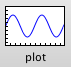
\includegraphics[scale=0.3]{plot_icon.png} to display a graph of the data.
    		\item Close the plot window by clicking the red `X' in the top right corner (or the red button on a Mac).
    		\item Take note of the output from the plot tool that has appeared in the \textbf{Command Window}.	The "plot" function is \emph{called} and is \emph{passed} all rows of the second column of \textbf{datacsv} as input.	
    	\end{itemize}
	\item From the \textbf{Command Window} use the plot function to plot the EMG data in the second column.
	\begin{itemize}
		\item Type the following:
		\begin{lstlisting}[style=Matlab-editor]
>> plot(datacsv(:,2));
		\end{lstlisting}
		\item You should see the same plot as before:
	\end{itemize}
	\begin{center}
		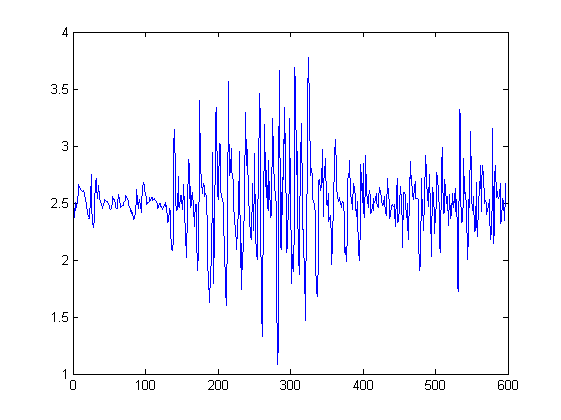
\includegraphics[width=\textwidth]{csvdata2.png}
	\end{center}
	\item Use the plot function to plot all six of the EMG channels on a single graph.  Keep this plot or \textbf{figure} open for later.
	\begin{itemize}
		\item Type the following:
		\begin{lstlisting}[style=Matlab-editor]
>> plot(datacsv(:,2:7));
		\end{lstlisting}		
		\item Notice how none of the EMG signals are centred around zero volts.
	\end{itemize}
	\begin{center}
		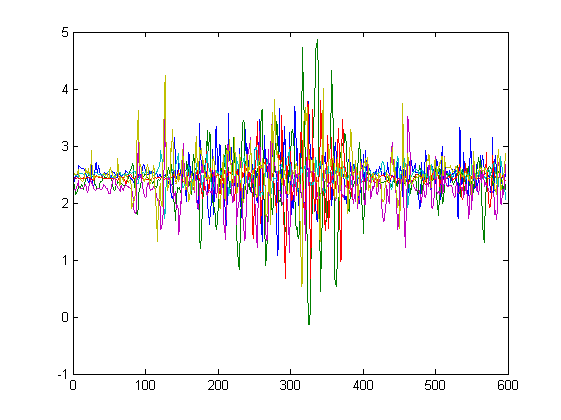
\includegraphics[width=\textwidth]{csvdata2-7.png}
	\end{center}
\end{enumerate}

\subsection{Processing the data}
You should now be getting the hang of how to access the contents of the data.  
We will now look at how to perform some basic analysis on these EMG data.  
Let us presume our aim is for the EMG data for each muscle to be plotted on separate graphs with time, in seconds, along the $x$-axis and the baseline corrected, rectified EMG amplitude signal, in mV, on the $y$-axis.  
From what we have seen from the data we have four main tasks to complete before we can display the results.
\begin{enumerate}
	\item Correct the first column of data from frame numbers to time, in seconds.	
	\item Baseline correct the EMG signals so that they are centred around zero.
	\item Rectify the EMG signals (convert values to positive amplitudes).
	\item Convert the volts (V) to mV for each EMG signal.
\end{enumerate}

\subsubsection*{Exercise}
\begin{enumerate}
	\item Duplicate the variable \textbf{datacsv} to create an identical new variable called \textbf{emgdata}.
	\begin{itemize}
		\item Copy the \textbf{datacsv} to a new variable \textbf{emgdata}.  Type the following:
		\begin{lstlisting}[style=Matlab-editor]
>> emgdata = datacsv;
		\end{lstlisting}		
	\end{itemize}
	
	\item Change the values in the first column to show the time in seconds.	
	\begin{itemize}
		\item Divide all of the values in column 1 by 200 to convert from frames to seconds. Type the following:
		\begin{lstlisting}[style=Matlab-editor]
>> emgdata(:,1) = datacsv(:,1)/200;
		\end{lstlisting}		
	\end{itemize}	
	
	\item Baseline correct the EMG signals by centring them at zero.
	\begin{itemize}
		\item Use MATLAB's \textbf{mean} function to find the mean value for each EMG signal.  Type:
		\begin{lstlisting}[style=Matlab-editor]
>> emgmeans = mean(datacsv(:,2:7));
		\end{lstlisting}		
		\item Subtract the mean value for the EMG signal from all of the values.  After pressing \textbf{Enter} to submit the first line, use the up arrow to prevent re-typing the whole line again.
		\begin{lstlisting}[style=Matlab-editor]
>> emgdata(:,2) = datacsv(:,2) - emgmeans(1);
>> emgdata(:,3) = datacsv(:,3) - emgmeans(2);
>> emgdata(:,4) = datacsv(:,4) - emgmeans(3);
>> emgdata(:,5) = datacsv(:,5) - emgmeans(4);
>> emgdata(:,6) = datacsv(:,6) - emgmeans(5);
>> emgdata(:,7) = datacsv(:,7) - emgmeans(6);
		\end{lstlisting}
	\end{itemize}
	\item Use the plot function to plot all six of the corrected EMG channels on a single graph in a \textbf{new figure}.
	\begin{itemize}
		\item Type the following:
		\begin{lstlisting}[style=Matlab-editor]
>> figure;
>> plot(emgdata(:,2:7));
		\end{lstlisting}		
		\item Notice how all of the EMG signals are now centred around zero volts.  
		You should be able to compare this plot with the plot from the previous exercise.			
	\end{itemize}		
	\begin{center}
		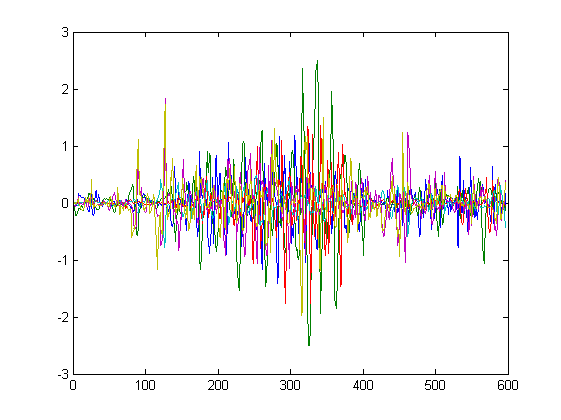
\includegraphics[width=\textwidth]{emgdata2-7.png}
	\end{center}
	\item Rectify all of the EMG data, i.e.~get only the magnitude of the signal, ignoring whether this is positive or negative.  This is also known as getting the \textbf{absolute} value.
	\begin{itemize}
		\item Close all of the current figures by using the \textbf{close} function.
		\begin{lstlisting}[style=Matlab-editor]
>> close all
		\end{lstlisting}
		\item Use the \textit{\textbf{fx}} button next to the command prompt ($>>$) to search for a MATLAB function to find the \textbf{absolute magnitude} of each EMG value.
		\item Use this function to rectify the EMG data.		
		\begin{lstlisting}[style=Matlab-editor]
>> emgdata(:,2:7) = abs(emgdata(:,2:7));
		\end{lstlisting}
	\end{itemize}
	\item Convert the EMG signals from volts (V) to millivolts (mV).
	\begin{itemize}
		\item Multiply all of the values in the EMG columns by 1000. 
		Type the following:
		\begin{lstlisting}[style=Matlab-editor]
>> emgdata(:,2:7) = emgdata(:,2:7)*1000;
		\end{lstlisting}
	\end{itemize}
	\item Plot the EMG data for the first EMG signal.  The time column should be on the $x$-axis and the EMG amplitude in mV should be the $y$-axis
	\begin{itemize}
		\item Use MATLAB's help documentation to find out how to plot the $x$ and $y$ data on the required axes.
		\item Use the \textbf{plot} function to plot the graph of EMG signal 1 (found in column 2 of the variable \textbf{emgdata}).
		\begin{lstlisting}[style=Matlab-editor]
>> plot(emgdata(:,1), emgdata(:,2));
		\end{lstlisting}		
		\item Using the help documentation find out how to add `Time (s)' as an $x$-axis label, `EMG amplitude (mV)' as a $y$-axis label and `The amplitude of Signal 1' as a title for the current plot.
		\begin{lstlisting}[style=Matlab-editor]
>> xlabel('Time (s)');
>> ylabel('EMG amplitude (mV)');
>> title('The EMG amplitude of signal 1');
		\end{lstlisting}	
		\begin{figure}[H]
\begin{center}
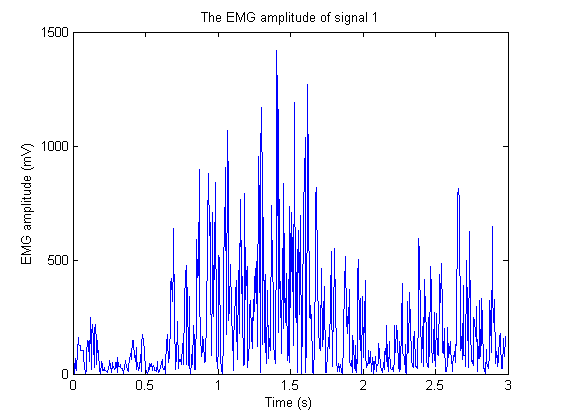
\includegraphics[width=\textwidth]{emgdata2.png}
\caption{A plot of the EMG amplitude of Signal 1 against time with axis labels and a title}
\label{fig:plot}
\end{center}
\end{figure}
		\item We could now repeat this process for each of the other five signals but this would be repetitive and time consuming.  
		Next week we will look at a number of ways to prevent the repetition and speed this process up.
	\end{itemize}
\end{enumerate}


\end{document}